\documentclass[UTF-8, a4paper, 12pt]{ctexart}

\usepackage[left=1in,right=1in,top=1.00in,bottom=1.00in]{geometry}% 页边距
\usepackage[colorlinks,linkcolor=blue,anchorcolor=blue,citecolor=green,CJKbookmarks=True]{hyperref}
\usepackage{CJK,CJKnumb}





% 首行缩进宏包
\usepackage{latexsym,bm}        % 处理数学公式中和黑斜体的宏包
\usepackage{amsmath,amssymb}     % AMSLaTeX宏包 用来排出更加漂亮的公式
\usepackage{graphicx}
\usepackage{cases}
\usepackage{pifont}
\usepackage{txfonts}
\usepackage{subfigure}
\usepackage{pdfpages}
\usepackage{listings}
\usepackage{xcolor}
\usepackage[subfigure]{tocloft}     % 模板中用了subfigure,不加此选项会产生冲突
\usepackage{inconsolata}
\usepackage{enumerate}
\usepackage{tcolorbox}% 文本框宏包
\usepackage{subfiles} %分章节编写
\CTEXsetup[format={\Large\bfseries}]{section}%设置章标题字号为Large,居左
\zihao{-4}\linespread{1.5}\selectfont
\renewcommand{\theequation}{\arabic{section}-\arabic{equation}}
\renewcommand{\thefigure}{\arabic{section}-\arabic{figure}}
\renewcommand{\thetable}{\arabic{section}-\arabic{table}}
%\renewcommand{\thefigure}{\thechapter-\arabic{figure}}
\renewcommand{\cftsecleader}{\cftdotfill{\cftdotsep}}
\renewcommand\contentsname{\centerline{Content}}
\renewcommand\listfigurename{{\centerline{Figures}}}
\renewcommand\listtablename{{\centerline{Tables}}}
\newcommand{\song}{\CJKfamily{song}}    % 宋体   (Windows自带simsun.ttf)
\renewcommand{\abstractname}{\textbf{\large {摘\quad 要}}} %更改摘要二字的样式

%%%%%%%%%%%%%%%%%%%%%%%
% 设置列表行距
\usepackage{enumitem}
\setenumerate[1]{itemsep=0pt,partopsep=0pt,parsep=\parskip,topsep=5pt}
\setitemize[1]{itemsep=0pt,partopsep=0pt,parsep=\parskip,topsep=5pt}
\setdescription{itemsep=0pt,partopsep=0pt,parsep=\parskip,topsep=5pt}
%%%%%%%%%%%%%%%%%%%%%%%
% -- text font --
% compile using Xelatex
%%%%%%%%%%%%%%%%%%%%%%%
% -- 中文字体 --
%\setCJKmainfont{Microsoft YaHei}  % 微软雅黑
%\setCJKmainfont{YouYuan}  % 幼圆
%\setCJKmainfont{NSimSun}  % 新宋体
%\setCJKmainfont{KaiTi}    % 楷体
%\setCJKmainfont{SimSun}   % 宋体
%\setCJKmainfont{FangSong}   % 仿宋
%\setCJKmainfont{SimHei}   % 黑体
 
% -- 英文字体 --
%\setmainfont{Times New Roman}
%\setmainfont{DejaVu Sans}
%\setmainfont{Latin Modern Mono}
%\setmainfont{Consolas}
\setmainfont{CMU Serif}

%%%%%%%%%%%%%%%%%%%%%%%
%  设置水印
%%%%%%%%%%%%%%%%%%%%%%%
%\usepackage{draftwatermark}         % 所有页加水印
%\usepackage[firstpage]{draftwatermark} % 只有第一页加水印
%\SetWatermarkText{Copyright(C) 2021. by HU S K}           % 设置水印内容
% \SetWatermarkText{\includegraphics{fig/ZJDX-WaterMark.eps}}         % 设置水印logo
%\SetWatermarkLightness{00.9}             % 设置水印透明度 0-1
%\SetWatermarkScale{0.4}                   % 设置水印大小 0-1
%%%%%%%%%%%%%%%%%%%%%%%




%%%%%%%%%%%%%%%%%%%%%%%%%%%%%%%%%%%%%%%%%%%
%用来设置附录中代码的样式
% 头文件
\usepackage{listings} 
\usepackage{fontspec}
\setmonofont{Consolas}
%\begin{lstlisting}[
%	language = matlab, numbers=left, 
%	numberstyle=\tiny,keywordstyle=\color{blue!70},
%	commentstyle=\color{red!50!green!50!blue!50},frame=shadowbox,
%	rulesepcolor=\color{red!20!green!20!blue!20},
%	basicstyle=\ttfamily,
%	]
%	
%\end{lstlisting}
%%%%%%%%%%%%%%%%%%%%%%%%%%%%%%%%%%%%%%%%%%%
% 更改标题形式
%\CTEXsetup[format={\Large\bfseries}]{section}%设置章标题字号为Large,居左
%\CTEXsetup[number={\chinese{section}}]{section}%section形式改为一,二,三,..
%\CTEXsetup[name={(,)}]{subsection}                                 
%\CTEXsetup[number={\chinese{subsection}}]{subsection}                %subsection形式改为(一,二,三,...)
              
%\CTEXsetup[number=\arabic{subsubsection}]{subsubsection}             %subsubsection形式改为1,2,3,...
%%%%%%%%%%%%%%%%%%%%%%%%%%%%%%%%%%%%%%%%%%%


\title{\bfseries \Huge  }
\author{}
\date{}

\begin{document}

\includepdf[pages={1}]{coverpage.pdf} %% 插入pdf

%\maketitle

%\thispagestyle{empty}
%\newpage
%\thispagestyle{empty}


    
\pagenumbering{Roman}    
\setcounter{page}{1}
\tableofcontents
\listoffigures
\listoftables
\newpage
\pagenumbering{arabic} 
\setcounter{page}{1}        %从下面开始编页,页脚格式为导言部分设置的格式



\section{实验目的}

\begin{enumerate}
    \item 基于提供的卷积神经网络示例代码,进行代码的优化,例如对GPU并行中的一些配置参数的优化。
    
    \item 或基于示例代码,开发U-Net等其他当前常用网络。 

\end{enumerate}

%\section{实验原理}

\section{CNN结构介绍}

在利用全连接神经网络处理大尺寸图像具有三个明显的缺点:
\begin{enumerate}
    \item 将图像展开为向量回丢失空间信息
    \item 参数过多效率低下,训练困难
    \item 大量参数会导致网络过拟合
\end{enumerate}

而使用卷积神经网络则不同,卷积神经网络中各层中的神经元是三位排列的:宽度、高度和深度。在卷积神经网络中国深度指的是激活数据体的第三个维度,而不是整个网络的深度。
\begin{figure}[htbp]
    \centering
    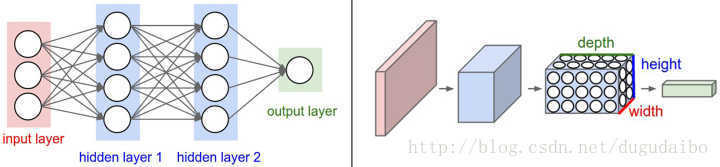
\includegraphics[width=15cm]{fig/f1.jpg}
    \caption{卷积神经网络和全连接神经网络的对比}
    \label{f1}
\end{figure}

图(\ref{f1})中左侧是一个三层的神经网络,右侧是一个卷积神经网络,将其神经元在三个维度(宽度,高度和深度)进行排列。卷积神经网络的每一层都将3D的输入数据变化为神经元3D的激活数据并输出。在图(\ref{f1})的右侧,红色的输入层代表输入图像,所以它的宽度和高度就是图像的宽度和高度,它的深度是3(代表了红、绿、蓝3种颜色通道),与红色相邻的蓝色部分是经过卷积和池化之后的激活值(也可以看做是神经元),后面是卷积池化层。



\section{构建卷积神经网络的层}

卷积神经网络主要由这几种层构成:输入层,卷积层,ReLU层,池化层和全连接层。通过将这些曾叠加起来,就可以构建一个完整的卷积神经网络。在实际应用中往往将卷积层与ReLU层共同称之为卷积层,因此卷积层经过卷积操作也是要经过激活函数的。具体来说,卷积层和全连接层对输入执行变换操作的时候,不仅会用到激活函数,还会用到很多参数,即神经元的权值$w$和偏差$b$;而ReLU层和池化层则是进行一个固定不变的函数操作。卷积层和全连接层中的参数会随着梯度下降被训练,这样卷积神经网络计算出的费雷评分就能和训练基中的每个图像的标签相吻合了。

\subsection{卷积层}
卷积层是构建卷积神经网络的核心层,他产生网络中的大部分计算量。
\subsubsection{卷积层的作用}

\begin{enumerate}
    \item 作为滤波器。卷积层的参数是由一些科学系的滤波器集合构成的,每个滤波器在高度和宽度上都比较小,但是深度和输入数据一致。
    \item 可以看作是一个神经元的输出。神经元只观察输入数据的一小部分,并且和空间上左右两边的所有神经元共享参数。
    \item 降低参数的数量。由于卷积有“权值共享”这样的特征,可以降低参数数量,达到降低计算开销,放置由于参数过多而造成过拟合。
\end{enumerate}

\subsubsection{感受野}

在处理图像这样的高维度输入时,让每一个神经元都与前一层中的所有神经元进行全连接是不现实的。相反,让每一个神经元只与输入数据的一个局部区域链接,该链接的空间大小叫做神经元的感受野(Receptive Field),其尺寸是一个超参数。在深度方向上,此连接的大小总是和输入量的深度相等。

\begin{figure}[htbp]
    \centering
    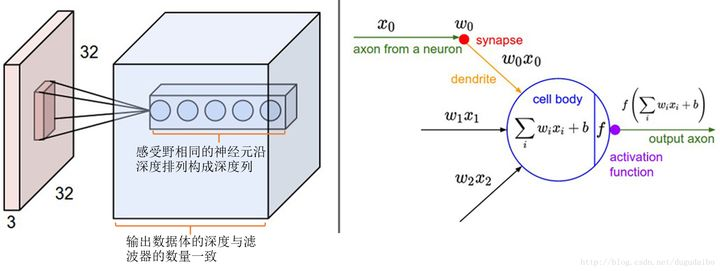
\includegraphics[width=15cm]{fig/f2.jpg}
    \caption{感受野的连接和尺寸说明}
    \label{f2}
\end{figure}

在图(\ref{f2})中展现的卷积神经网络的一部分,其中的红色为输入数据,假设输入数据体尺寸为$[32\times 32\times 3]$,如果感受野(或滤波器尺寸)是$5\times 5$,那么卷积层中的每个神经元会有输入数据体中$[5\times 5\times 3]$区域的权重,$共5\times 5\times 3=75$个权重。注意这个连接在深度维度上的大小必须为3,和输入数据体的深度一致。其中还有一点需要注意,对应一个感受野有75个权重,这75个权重是通过学习进行更新的,所以很大程度上这些权值之间是不相等。在这里相当于前面的每一个层对应一个传统意义上的卷积模板,每一层与自己卷积模板做完卷积之后,再将各个层的结果加起来,再加上一个偏置。

\subsubsection{神经元的空间排列}

感受野讲解了卷积层中每个神经元与输入数据体之间的连接方式,但是尚未讨论输出数据体中神经元的数量,以及它们的排列方式。3个超参数控制着输出数据体的尺寸:深度(depth),步长(stride)和零填充(zero-padding)。

\begin{enumerate}
    \item 输出数据体的深度。它是一个超参数,和使用的滤波器的数量一致,而每个滤波器在输入数据中寻找一些不同的东西,即图像的某些特征。如图(\ref{f2})所示,将沿着深度方向排列、感受野相同的神经元集合称为深度列(depth column)
    \item 在滑动滤波器的时候,必须指定步长。当步长为1,滤波器每次移动1个像素;当步长为2,滤波器滑动时每次移动2个像素,当然步长也可以是不常用的3,或者更大的数字,但这些在实际中很少使用)。这个操作会让输出数据体在空间上变小。
    \item 有时候将输入数据体用0在边缘处进行填充是很方便的。这个零填充(zero-padding)的尺寸是一个超参数。零填充有一个良好性质,即可以控制输出数据体的空间尺寸(最常用的是用来保持输入数据体在空间上的尺寸,使得输入和输出的宽高都相等)。
\end{enumerate}

输出数据体在空间上的尺寸$W_2\times H_2\times D_2$可以通过输入数据尺寸$W_1\times H_1\times D_1$,卷积层中神经元的感受野尺寸$F$,步长$S$,滤波器数量$K$和零填充数量$P$计算得到。
\begin{gather}
    W_2=\frac{W_1-F+2P}{S}+1
    \\
   H_2=\frac{H_1-F+2P}{S}+1\\
D_2=K
\end{gather}
一般来说,当步长$S=1$时,零填充的值为$P=(F-1)/2$,这样就能保证输入和输出数据体有相同的空间尺寸。

\subsubsection{权值共享}

在卷积层中权值共享是用来控制参数的数量。假如在一个卷积核中,每一个感受野采用的都是不同的权重值(卷积核的值不同),那么这样的网络中参数数量将是十分巨大的。

权值共享是基于这样的一个合理的假设:如果一个特征在计算某个空间位置 $(x_1,y_1)$的时候有用,那么它在计算另一个不同位置 $(x_2,y_2) $的时候也有用。基于这个假设,可以显著地减少参数数量。换言之,就是将深度维度上一个单独的2维切片看做深度切片(depth slice),比如一个数据体尺寸为$[55\times 55\times 96]$的就有96个深度切片,每个尺寸为$[55\times 55]$,其中在每个深度切片上的结果都使用同样的权重和偏差获得的。在这样的参数共享下,假如一个例子中的第一个卷积层有96个卷积核,那么就有96个不同的权重集了,一个权重集对应一个深度切片,如果卷积核的大小是$ 11\times 11$的,图像是RGB为3通道,那么就共有$96\times 11\times 11\times 3=34848$个不同的权重,总共有34944个参数(因为要加上96个偏差),并且在每个深度切片中的$55\times 55 $的结果使用的都是同样的参数。

在反向传播的时候,都要计算每个神经元对它的权重的梯度,但是需要把同一个深度切片上的所有神经元对权重的梯度累加,这样就得到了对共享权重的梯度。这样,每个切片只更新一个权重集。这样做的原因可以通过图(\ref{f3})进行解释。

\begin{figure}[htbp]
    \centering
    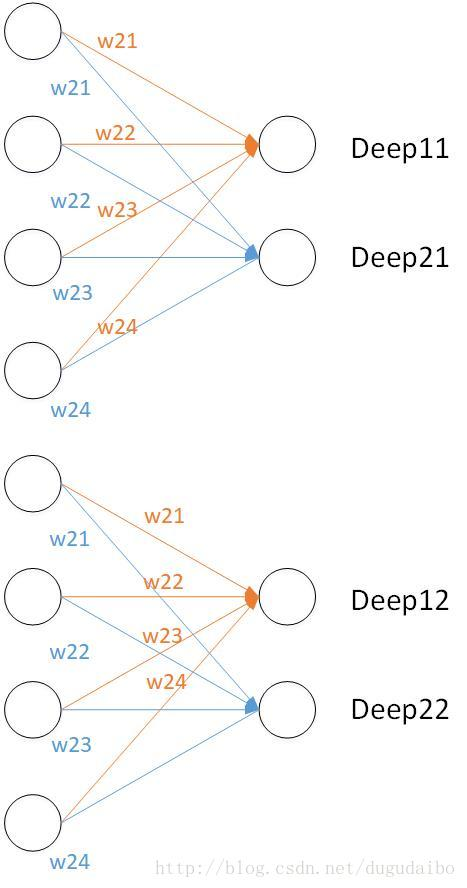
\includegraphics[width=5cm]{fig/f3.jpg}
    \caption{将卷积层用全连接层的形式表示}
    \label{f3}
\end{figure}

如图(\ref{f3})所示,左侧的神经元是将每一个感受野展开为一列之后串联起来(就是展开排成一列,同一层神经元之间不连接)。右侧的 Deep1i 是深度为1的神经元的第 i 个, Deep2i 是深度为2的神经元的第 i 个,同一个深度的神经元的权值都是相同的,黄色的都是相同的(上面4个与下面4个的参数相同),蓝色都是相同的。所以现在回过头来看上面说的卷积神经网络的反向传播公式对梯度进行累加求和也是基于这点考虑(同一深度的不同神经元共用一组参数,所以累加);而每个切片只更新一个权重集的原因也是这样的,因为从图3 中可以看到,不同深度的神经元不会公用相同的权重,所以只能更新一个权重集。

\subsubsection{卷积层的超参数及选择}

由于参数共享,每个滤波器包含$F\times F \times D_1$个权重,卷积层一共有$F\times F\times D_1\times K$个权重和$K$个偏置。在输出数据体中,第$d$个深度切牌(空间尺寸为$W_2\times H_2$),用第$d$个滤波器和输入数据进行有效卷积运算的结果(使用步长$S$),最后在加上第$d$个偏差。

\subsubsection{实现卷积的操作}

\begin{enumerate}
    \item 矩阵乘法实现卷积:
    
    卷积运算本质上就是在滤波器和输入数据的局部区域间做点积。卷积层的常用实现方式就是利用这一点,将卷积层的前向传播变成一个巨大的矩阵乘法。

    \item $1\times 1$卷积:
    
    一些论文中使用了$1\times 1$的卷积,这个方法最早是在论文Network in Network中出现。人们刚开始看见这个$1\times 1$卷积的时候比较困惑,尤其是那些具有信号处理专业背景的人。因为信号是2维的,所以$1\times 1$卷积就没有意义。但是,在卷积神经网络中不是这样,因为这里是对3个维度进行操作,滤波器和输入数据体的深度是一样的。比如,如果输入是$[32\times 32\times 3]$,那么$1\times 1$卷积就是在高效地进行3维点积;另外的一种想法是将这种卷积的结果看作是全连接层的一种实现方式。

    \item 扩张卷积:
    
    最近一个研究给卷积层引入了一个新的叫扩张(dilation)的超参数。到目前为止,我们只讨论了卷积层滤波器是连续的情况。但是,让滤波器中元素之间有间隙也是可以的,这就叫做扩张,如图(\ref{f5})所示。
    \begin{figure}[htbp]
        \centering
        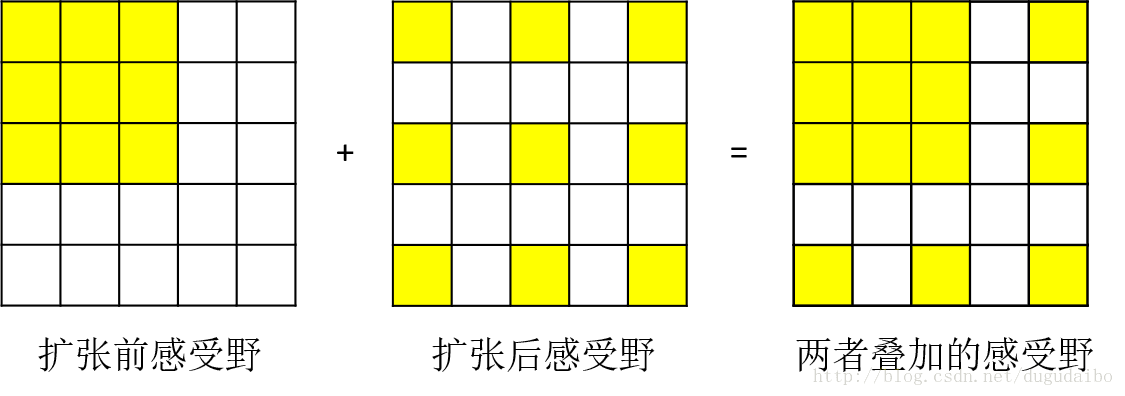
\includegraphics[width=15cm]{fig/f5.jpg}
        \caption{扩张卷积示意图及扩张前后的叠加效果}
        \label{f5}
    \end{figure}
\end{enumerate}

\subsection{池化层}

通常在连续的卷积层之间会周期性地插入一个池化层。它的作用是逐渐降低数据体的空间尺寸,这样的话就能减少网络中参数的数量,使得计算资源耗费变少,也能有效控制过拟合。汇聚层使用 MAX 操作,对输入数据体的每一个深度切片独立进行操作,改变它的空间尺寸。最常见的形式是汇聚层使用尺寸$2\times 2$的滤波器,以步长为2来对每个深度切片进行降采样,将其中75\%的激活信息都丢掉。每个MAX操作是从4个数字中取最大值(也就是在深度切片中某个$2\times 2$的区域),深度保持不变。

\subsection{归一化层}
在卷积神经网络的结构中,提出了很多不同类型的归一化层,有时候是为了实现在生物大脑中观测到的抑制机制。但是这些层渐渐都不再流行,因为实践证明它们的效果即使存在,也是极其有限的。

\subsection{全连接层}
全连接层和常规神经网络中一样,它们的激活可以先用矩阵乘法,再加上偏差。

\subsubsection{将卷积层转化为全连接层}
对于任一个卷积层,都存在一个能实现和它一样的前向传播函数的全连接层。该全连接层的权重是一个巨大的矩阵,除了某些特定块(感受野),其余部分都是零;而在非 0 部分中,大部分元素都是相等的(权值共享)。如果把全连接层转化成卷积层,以输出层的 Deep11 为例,与它有关的输入神经元只有上面四个,所以在权重矩阵中与它相乘的元素,除了它所对应的4个,剩下的均为0,这也就解释了为什么权重矩阵中有为零的部分;另外要把“将全连接层转化成卷积层”和“用矩阵乘法实现卷积”区别开,这两者是不同的,后者本身还是在计算卷积,只不过将其展开为矩阵相乘的形式,并不是”将全连接层转化成卷积层”,所以除非权重中本身有零,否则用矩阵乘法实现卷积的过程中不会出现值为0的权重。

\subsubsection{将全连接层转化为卷积层}
任何全连接层都可以被转化为卷积层。比如,一个$K=4096$的全连接层,输入数据体的尺寸是$ 7\times 7\times 5127\times 7\times 512$,这个全连接层可以被等效地看做一个$F=7,P=0,S=1,K=4096,F=7,P=0,S=1,K=4096$的卷积层。换句话说,就是将滤波器的尺寸设置为和输入数据体的尺寸设为一致的。因为只有一个单独的深度列覆盖并滑过输入数据体,所以输出将变成$1\times 1\times 40961\times 1\times 4096$,这个结果就和使用初始的那个全连接层相同。对于其中的一个卷积滤波器,这个滤波器的的深度为512,因此虽然这个卷积滤波器的输出只有1个,但是它的权重有$7\times 7\times 5127\times 7\times 512$,相当于卷积滤波器的输出为一个神经元,这个神经元与上一层的所有神经元相连接,而这样与前一层所有神经元相连接的神经元一共有4096个,即为一个全连接网络。

在上述的两种变换中,将全连接层转化为卷积层在实际运用中更加有用。假设一个卷积神经网络的输入是$224\times 224\times 3$的图像,一系列的卷积层和汇聚层将图像数据变为尺寸为$7\times 7\times 512$的激活数据体(在AlexNet中就是这样,通过使用5个汇聚层来对输入数据进行空间上的降采样,每次尺寸下降一半,所以最终空间尺寸为$224/2/2/2/2/2=7$)。从这里可以看到,AlexNet使用了两个尺寸为4096的全连接层,最后一个有1000个神经元的全连接层用于计算分类评分。我们可以将这3个全连接转化为3个卷积层:
\begin{enumerate}
    \item 针对第一个连接区域是$[7\times 7\times 512]$的全连接层,令其滤波器尺寸为$F=7$,这样输出数据体就为$[1\times 1\times 4096]$了。
    \item  针对第二个全连接层,令其滤波器尺寸为$F=1$,这样输出数据体为$[1\times 1\times 4096]$。
    \item 对最后一个全连接层也做类似的,令其$F=1$,最终输出为$[1\times 1\times 1000]$。
\end{enumerate}

这样做的目的是让卷积网络在一张更大的输入图片上滑动,得到多个输出,这样的转化可以让我们在单个向前传播的过程中完成上述的操作。

\section{卷积神经网络结构}
卷积神经网络通常是由三种层构成:卷积层,汇聚层(除非特别说明,一般就是最大值汇聚)和全连接层(简称FC)。ReLU激活函数也应该算是是一层,它逐元素地进行激活函数操作,常常将它与卷积层看作是同一层。

\subsection{层的排列规律}
卷积神经网络最常见的形式就是将一些卷积层和ReLU层放在一起,其后紧跟汇聚层,然后重复如此直到图像在空间上被缩小到一个足够小的尺寸,在某个地方过渡成成全连接层也较为常见。最后的全连接层得到输出,比如分类评分等。换句话说,最常见的卷积神经网络结构如下:
$$ INPUT\rightarrow[CONV\rightarrow RELU]*N\rightarrow [POOL?]*M\rightarrow[FC\rightarrow RELU]*K\rightarrow FC$$

其中$*$指的是重复次数,$POOL?$指的是一个可选的汇聚层。其中$N >=0$,通常$N<=3,M>=0,K>=0$,通常$K<3$。
\subsection{卷积层大小的选择}

几个小滤波器卷积层的组合比一个大滤波器卷积层好。假设一层一层地重叠了3个$3\times 3$的卷积层(层与层之间有非线性激活函数)。在这个排列下,第一个卷积层中的每个神经元都对输入数据体有一个$3\times 3$的视野。第二个卷积层上的神经元对第一个卷积层有一个$3\times 3$的视野,也就是对输入数据体有$5\times 5$的视野。同样,在第三个卷积层上的神经元对第二个卷积层有$3\times 3$的视野,也就是对输入数据体有$7\times 7$的视野。假设不采用这3个$3\times 3$的卷积层,二是使用一个单独的有$7\times 7$的感受野的卷积层,那么所有神经元的感受野也是$7\times 7$,但是就有一些缺点。首先,多个卷积层与非线性的激活层交替的结构,比单一卷积层的结构更能提取出深层的更好的特征。其次,假设所有的数据有C个通道,那么单独的7x7卷积层将会包含$C\times(7\times 7\times C)=49C^2$个参数,而3个$7\times 7$的卷积层的组合仅有$3\times C\times(3\times 3\times C)=27C^2$个参数。直观说来,最好选择带有小滤波器的卷积层组合,而不是用一个带有大的滤波器的卷积层。前者可以表达出输入数据中更多个强力特征,使用的参数也更少。唯一的不足是,在进行反向传播时,中间的卷积层可能会导致占用更多的内存。

\subsection{层的尺寸设置规律}
\begin{enumerate}
    \item 输入层
    
  大小应为2的幂次或可多次被2整除。常用数字包括32(比如CIFAR-10),64,96(比如STL-10)或224(比如ImageNet卷积神经网络),384和512。
  \item 卷积层
  
  应该使用小尺寸滤波器,使用步长$S=1$。还有一点非常重要,就是对输入数据进行零填充,这样卷积层就不会改变输入数据在空间维度上的尺寸。比如,当$F=3$,那就使用$P=1$来保持输入尺寸。当$F=5,P=2$,一般对于任意$F$,当$P=(F-1)/2$的时候能保持输入尺寸。如果必须使用更大的滤波器尺寸,通常只用在第一个面对原始图像的卷积层上。

  \item 汇聚层
  
  负责对输入数据的空间维度进行降采样。最常用的设置是用用$2\times 2$感受野(即$F=2$)的最大值汇聚,步长为$2(S=2)$。注意这一操作将会把输入数据中75\%的激活数据丢弃(因为对宽度和高度都进行了2的降采样)。另一个不那么常用的设置是使用$3\times 3$的感受野,步长为2。最大值汇聚的感受野尺寸很少有超过3的,因为汇聚操作过于激烈,易造成数据信息丢失,这通常会导致算法性能变差。
\end{enumerate}



\section{CNN计算上的考量}
在构建卷积神经网络结构时,最大的瓶颈是内存瓶颈,所以如何降低内存消耗量是一个值得思考的问题。三种内存占用来源:

\begin{enumerate}
    \item 来自中间数据体尺寸:
    
    卷积神经网络中的每一层中都有激活数据体的原始数值,以及损失函数对它们的梯度(和激活数据体尺寸一致)。通常,大部分激活数据都是在网络中靠前的层中(比如第一个卷积层)。在训练时,这些数据需要放在内存中,因为反向传播的时候还会用到。但是在测试时可以聪明点:让网络在测试运行时候每层都只存储当前的激活数据,然后丢弃前面层的激活数据,这样就能减少巨大的激活数据量。这实际上是底层问题,在编写框架的过程中,设计者会进行这方面的考虑。
    \item 来自参数尺寸:
    
    即整个网络的参数的数量,在反向传播时它们的梯度值,以及使用momentum、Adagrad或RMSProp等方法进行最优化时的每一步计算缓存。因此,存储参数向量的内存通常需要在参数向量的容量基础上乘以3或者更多。

    \item 卷积神经网络实现还有各种零散的内存占用,比如成批的训练数据,扩充的数据等等。
\end{enumerate}

一旦对于所有这些数值的数量有了一个大略估计(包含激活数据,梯度和各种杂项),数量应该转化为以GB为计量单位。把这个值乘以4,得到原始的字节数(因为每个浮点数占用4个字节,如果是双精度浮点数那就是占用8个字节),然后多次除以1024分别得到占用内存的KB,MB,最后是GB计量。如果你的网络工作得不好,一个常用的方法是降低批尺寸(batch size),因为绝大多数的内存都是被激活数据消耗掉了。
\section{实验过程}

\subsection{\colorbox[gray]{0.9}{\texttt{Seq\_CNN\_course}}代码分析}
对\colorbox[gray]{0.9}{\texttt{Seq\_CNN\_course}}中的代码进行分析。在\colorbox[gray]{0.9}{\texttt{Seq\_CNN\_course}}中,主要由以下几个部分组成:

1. \colorbox[gray]{0.9}{\texttt{drv\_cnn}}:

此部分是卷积神经网络的驱动程序,是顶层程序。

\bigskip
2. \colorbox[gray]{0.9}{\texttt{Activation\_layer}}:

此函数是激活层,含有激活函数。
    所谓激活函数,就是在人工神经网络的神经元上运行的函数,负责将神经元的输入映射到输出端。

激活函数对于人工神经网络模型去学习、理解非常复杂和非线性的函数来说具有十分重要的作用。它们将非线性特性引入到我们的网络中。且在本程序中,采用的激活函数

在本程序中,在类中定义了三种激活函数,分别为$\tanh$函数,ReLU函数,Sigmoid函数,并分别定义了三种激活函数的梯度函数。下面对这三种激活函数作一简单介绍。\begin{itemize}
    \item Sigmoid函数:Sigmoid函数是一个在生物学中常见的S型函数,也称为S型生长曲线。在信息科学中,由于其单增以及反函数单增等性质,Sigmoid函数常被用作神经网络的阈值函数,将变量映射到0至1之间。公式如下,其函数图像如图(\ref{sigmoid})所示。\begin{equation}
        f(x)=\frac{1}{1+e^{-x}}
    \end{equation}
    \begin{figure}[htbp]
        \centering
        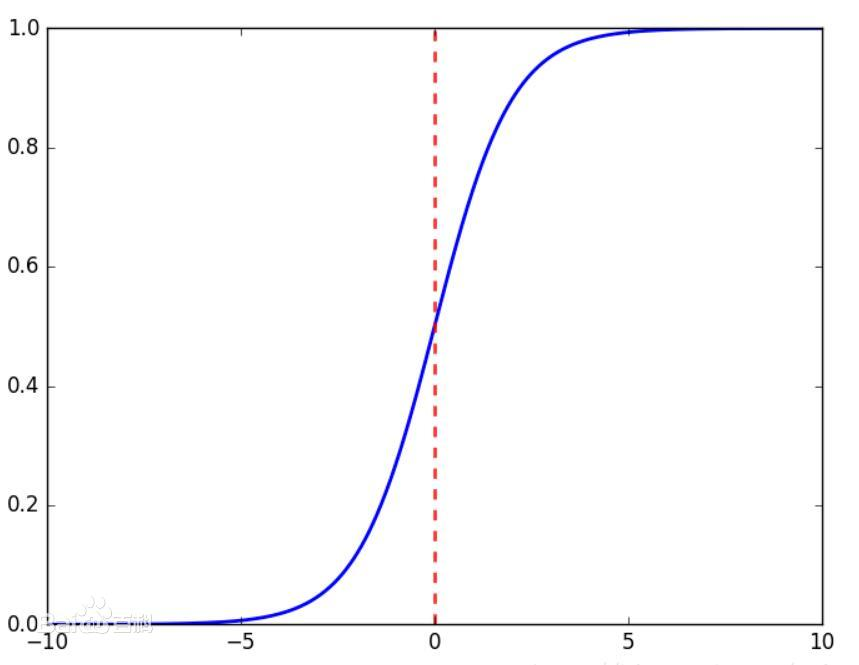
\includegraphics[width=6cm]{fig/sigmoid.jpg}
        \caption{Sigmoid 函数图像}
        \label{sigmoid}
    \end{figure}
    \item $\tanh$函数:$\tanh$是双曲函数中的一个,$\tanh()$为双曲正切。在数学中,双曲正切$\tanh$是由基本双曲函数双曲正弦和双曲余弦推导而来。公式如下,其函数图像如图(\ref{tanh})所示。\begin{equation}
        f(x)=\frac{e^x-e^{-x}}{e^x+e^{-x}}
    \end{equation}
    \begin{figure}[htbp]
        \centering
        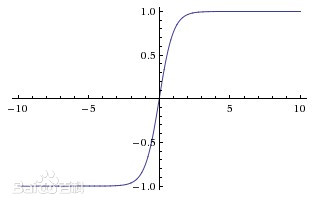
\includegraphics[width=6cm]{fig/tanh.jpg}
        \caption{$\tanh$函数图像}
        \label{tanh}
    \end{figure}

    \item ReLU函数:Relu激活函数(The Rectified Linear Unit),用于隐层神经元输出。公式如下,其函数图像如图(\ref{relu})所示。\begin{equation}
        f(x)=\max(0,x)
    \end{equation}
    \begin{figure}[htbp]
        \centering
        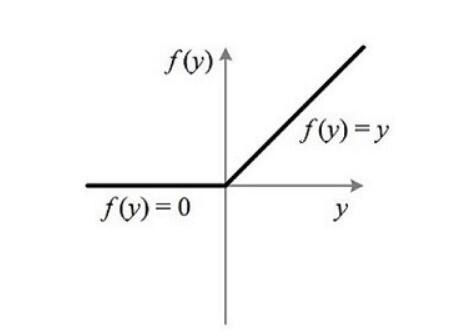
\includegraphics[width=6cm]{fig/relu.jpg}
        \caption{ReLU函数图像}
        \label{relu}
    \end{figure}
\end{itemize}

在程序\colorbox[gray]{0.9}{\texttt{activation\_layer.cc}}中,利用的激活函数为Tanh,以此来实现非线性效应。


\bigskip
3. \colorbox[gray]{0.9}{\texttt{convolutional\_layer}}

此部分为卷积层,在头文件中定义了卷积核大小,步长,零填充尺寸等超参数。在.cc文件中,主要有三个函数:初始化权重,前向卷积和后向卷积。

\bigskip
4. \colorbox[gray]{0.9}{\texttt{pooling\_layer}}

此部分为池化层,同样在头文件中定义了一些超参数,与卷积层中的头文件几乎一样,只是仅仅少了几个超参数。
在本池化层,采用的是最常见的最大池化层,池化层的目的主要是模仿人的视觉系统对数据进行降维,用更高层次的特征表示图像。



\bigskip
5. \colorbox[gray]{0.9}{\texttt{fully\_connected\_layer}}

此部分为全连接层。同样的,在头文件中定义了一些超参数,在.cc文件中,主要有三个函数:初始化权重,前向和后向传播函数。

当来到了全连接层之后,可以理解为一个简单的多分类神经网络(如:BP神经网络),通过softmax函数得到最终的输出。整个模型训练完毕。两层之间所有神经元都有权重连接,通常全连接层在卷积神经网络尾部。也就是跟传统的神经网络神经元的连接方式是一样的。

\bigskip
6. \colorbox[gray]{0.9}{\texttt{softmax\_layer}}

本层为softmax层,softmax层只是对神经网络的输出结果进行了一次换算,将输出结果用概率的形式表现出来。
\subsection{\colorbox[gray]{0.9}{\texttt{Cuda\_CNN\_ptr}}代码分析比较}


\subsubsection{CUDA简介}
CUDA是NVIDIA公司所开发的GPU编程模型,它提供了GPU编程的简易接口,基于CUDA编程可以构建基于GPU计算的应用程序。CUDA提供了对其它编程语言的支持,如C/C++,Python,Fortran等语言。基于CUDA编程可以利用GPUs的并行计算引擎来更加高效地解决比较复杂的计算难题。近年来,GPU最成功的一个应用就是深度学习领域,基于GPU的并行计算已经成为训练深度学习模型的标配。目前,最新的CUDA版本为CUDA 9。

GPU并不是一个独立运行的计算平台,而需要与CPU协同工作,可以看成是CPU的协处理器,因此当我们在说GPU并行计算时,其实是指的基于CPU+GPU的异构计算架构。在异构计算架构中,GPU与CPU通过PCIe总线连接在一起来协同工作,CPU所在位置称为为主机端(host),而GPU所在位置称为设备端(device),如下图(\ref{f11})所示。

\begin{figure}[htbp]
    \centering
    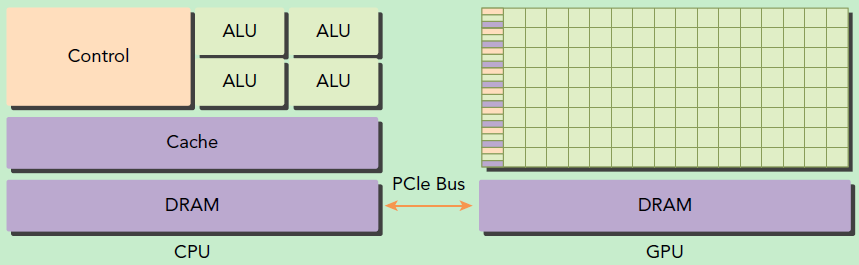
\includegraphics[width=16cm]{fig/f11.png}
    \caption{基于CPU+GPU的异构计算}
    \label{f11}
\end{figure}

可以看到GPU包括更多的运算核心,其特别适合数据并行的计算密集型任务,如大型矩阵运算,而CPU的运算核心较少,但是其可以实现复杂的逻辑运算,因此其适合控制密集型任务。另外,CPU上的线程是重量级的,上下文切换开销大,但是GPU由于存在很多核心,其线程是轻量级的。因此,基于CPU+GPU的异构计算平台可以优势互补,CPU负责处理逻辑复杂的串行程序,而GPU重点处理数据密集型的并行计算程序,从而发挥最大功效。



\subsubsection{CUDA编程模型基础}
在给出CUDA的编程实例之前,这里先对CUDA编程模型中的一些概念及基础知识做个简单介绍。CUDA编程模型是一个异构模型,需要CPU和GPU协同工作。在CUDA中,host和device是两个重要的概念,我们用host指代CPU及其内存,而用device指代GPU及其内存。CUDA程序中既包含host程序,又包含device程序,它们分别在CPU和GPU上运行。同时,host与device之间可以进行通信,这样它们之间可以进行数据拷贝。典型的CUDA程序的执行流程如下:

\begin{enumerate}
    \item 分配host内存,并进行数据初始化;
    \item 分配device内存,并从host将数据拷贝到device上;
    \item 调用CUDA的核函数在device上完成指定的运算;
    \item 将device上的运算结果拷贝到host上;
    \item 释放device和host上分配的内存。
\end{enumerate}

上面流程中最重要的一个过程是调用CUDA的核函数来执行并行计算,kernel是CUDA中一个重要的概念,kernel是在device上线程中并行执行的函数,核函数用\colorbox[gray]{0.9}{\texttt{\_\_global\_\_}}符号声明,在调用时需要用\colorbox[gray]{0.9}{\texttt{<<<grid, block>>>}}来指定kernel要执行的线程数量,在CUDA中,每一个线程都要执行核函数,并且每个线程会分配一个唯一的线程号thread ID,这个ID值可以通过核函数的内置变量\colorbox[gray]{0.9}{\texttt{threadIdx}}来获得。

由于GPU实际上是异构模型,所以需要区分host和device上的代码,在CUDA中是通过函数类型限定词开区别host和device上的函数,主要的三个函数类型限定词如下:
\begin{itemize}
    \item \colorbox[gray]{0.9}{\texttt{\_\_global\_\_}}:在device上执行,从host中调用(一些特定的GPU也可以从device上调用),返回类型必须是\colorbox[gray]{0.9}{\texttt{void}},不支持可变参数参数,不能成为类成员函数。注意用\colorbox[gray]{0.9}{\texttt{\_\_global\_\_}}定义的kernel是异步的,这意味着host不会等待kernel执行完就执行下一步。
    \item \colorbox[gray]{0.9}{\texttt{\_\_device\_\_}}:在device上执行,单仅可以从device中调用,不可以和\colorbox[gray]{0.9}{\texttt{\_\_global\_\_}} 同时用。
    \item \colorbox[gray]{0.9}{\texttt{\_\_host\_\_}}:在host上执行,仅可以从host上调用,一般省略不写,不可以和\colorbox[gray]{0.9}{\texttt{\_\_global\_\_}}同时用,但可和\colorbox[gray]{0.9}{\texttt{\_\_device\_\_}},此时函数会在device和host都编译。
\end{itemize}

要深刻理解kernel,必须要对kernel的线程层次结构有一个清晰的认识。首先GPU上很多并行化的轻量级线程。kernel在device上执行时实际上是启动很多线程,一个kernel所启动的所有线程称为一个网格(grid),同一个网格上的线程共享相同的全局内存空间,grid是线程结构的第一层次,而网格又可以分为很多线程块(block),一个线程块里面包含很多线程,这是第二个层次。线程两层组织结构如下图所示,这是一个gird和block均为2-dim的线程组织。grid和block都是定义为
\colorbox[gray]{0.9}{\texttt{dim3}}
类型的变量,
\colorbox[gray]{0.9}{\texttt{dim3}}
可以看成是包含三个无符号整数$(x,y,z)$成员的结构体变量,在定义时,缺省值初始化为1。因此grid和block可以灵活地定义为1-dim,2-dim以及3-dim结构,对于图(\ref{f13})中结构(主要水平方向为x轴),定义的\colorbox[gray]{0.9}{\texttt{grid}}和\colorbox[gray]{0.9}{\texttt{block}}如下所示,kernel在调用时也必须通过执行配置\colorbox[gray]{0.9}{\texttt{<<<grid, block>>>}}来指定kernel所使用的线程数及结构。
\begin{lstlisting}[
	language = matlab, numbers=left, 
	numberstyle=\tiny,keywordstyle=\color{blue!70},
	commentstyle=\color{red!50!green!50!blue!50},frame=shadowbox,
	rulesepcolor=\color{red!20!green!20!blue!20},
	basicstyle=\ttfamily,
	]
dim3 grid(3, 2);
dim3 block(5, 3);
kernel_fun<<< grid, block >>>(prams...);
\end{lstlisting}

\begin{figure}[htbp]
    \centering
    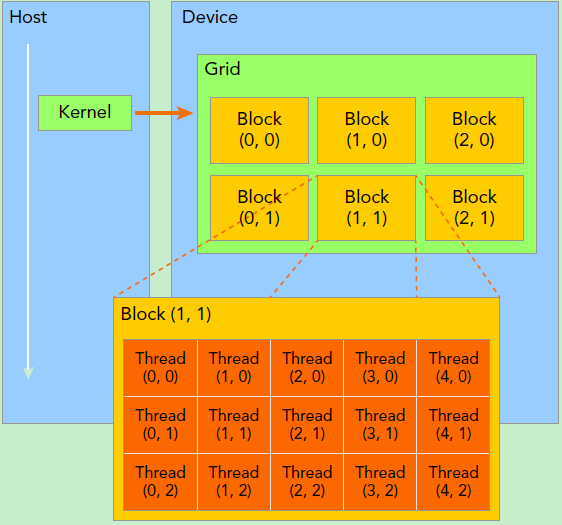
\includegraphics[width=10cm]{fig/f13.png}
    \caption{Kernel上的两层线程组织结构(2-dim)}
    \label{f13}
\end{figure}

所以,一个线程需要两个内置的坐标变量(blockIdx,threadIdx)来唯一标识,它们都是\colorbox[gray]{0.9}{\texttt{dim3}}类型变量,其中\colorbox[gray]{0.9}{\texttt{blockIdx}}指明线程所在grid中的位置,而\colorbox[gray]{0.9}{\texttt{threaIdx}}指明线程所在block中的位置,如图(\ref{f13})中的Thread(1,1)满足:

\begin{lstlisting}[
	language = matlab, numbers=left, 
	numberstyle=\tiny,keywordstyle=\color{blue!70},
	commentstyle=\color{red!50!green!50!blue!50},frame=shadowbox,
	rulesepcolor=\color{red!20!green!20!blue!20},
	basicstyle=\ttfamily,
	]
threadIdx.x = 1
threadIdx.y = 1
blockIdx.x = 1
blockIdx.y = 1
\end{lstlisting}

一个线程块上的线程是放在同一个流式多处理器(SM)上的,但是单个SM的资源有限,这导致线程块中的线程数是有限制的,现代GPUs的线程块可支持的线程数可达1024个。有时候,我们要知道一个线程在blcok中的全局ID,此时就必须还要知道block的组织结构,这是通过线程的内置变量blockDim来获得。它获取线程块各个维度的大小。对于一个2-dim的$block(D_x,D_y)$ ,线程$(x,y)$的ID值为$(x+y\times D_x)$,如果是3-dim的$block(D_x,D_y,D_z)$ ,线程$(x,y,z)$的ID值为$(x+y\times D_x+z\times D_z\times D_y)$。另外线程还有内置变量\colorbox[gray]{0.9}{\texttt{gridDim}},用于获得网格块各个维度的大小。

\subsubsection{代码分析比较}

对\colorbox[gray]{0.9}{\texttt{Cuda\_CNN\_ptr}}中的代码进行分析。并与\colorbox[gray]{0.9}{\texttt{Seq\_CNN\_course}}中的代码进行比较,\colorbox[gray]{0.9}{\texttt{Cuda\_CNN\_ptr}}程序主要由以下几个部分组成:

\begin{enumerate}
    \item \colorbox[gray]{0.9}{\texttt{drv\_cnn}}
    \item \colorbox[gray]{0.9}{\texttt{Activation\_layer}}
    \item \colorbox[gray]{0.9}{\texttt{convolutional\_layer}}
    \item \colorbox[gray]{0.9}{\texttt{pooling\_layer}}
    \item \colorbox[gray]{0.9}{\texttt{fully\_connected\_layer}}
    \item \colorbox[gray]{0.9}{\texttt{softmax\_layer}}
\end{enumerate}

此程序主页也是由此六大程序组成,分别为顶层程序、激活层、卷积层、池化层、全连接层和softmax层组成,其结构与\colorbox[gray]{0.9}{\texttt{Seq\_CNN\_course}}基本相同,可以认为结构基本一样,只是在每一层的具体实现上,利用了CUDA编程,利用GPU并行加速程序运行时间。





\subsection{更改网络超参数(炼丹)}

\subsubsection{学习率调参}

更改\colorbox[gray]{0.9}{\texttt{Cuda\_CNN\_ptr}}程序中的网络学习率。

首先令学习率为$learning\_rate=0.01\times \sqrt{batch\_size\_train}=0.01\sqrt{240}$,对程序进行测试。然后再令$learning\_rate=0.01\times k\times \sqrt{240},\ k=2,3,\cdots$,分别进行测试,并分别统计训练时间、准确率、测试时间,得到结果如下表(\ref{learning_rate})所示:
\begin{table}[htbp]
    \centering
    \caption{学习率测试结果}\label{learning_rate}
    \begin{tabular}{c|cccccccc}
        \hline
        $k$&1&2&3&4&5&10&20&30\\
        \hline 
        训练时间(ms)&266.73&265.86&268.17&265.77&268.22&265.63&267.40&267.28\\
        测试时间(ms)&41.76&41.93&41.90&42.04&41.98&42.25&42.16&41.73\\
        准确率(\%)&94.58& 95.98&96.73&96.71&96.77&96.94&95.68&20.32\\
        \hline  
        
    \end{tabular}
\end{table}

通过上表(\ref{learning_rate})可以看到,学习率的改变对训练时间和测试时间基本没有影响,但是对准确率有很大影响,当$k=10$学习率为$0.1\sqrt{240}$的时候,可以看到准确率是最高的,相比学习率为$0.01\sqrt{240}$时,提高了2.5个百分点,可见提高效果显著。

但是当学习率持续增加时,可以看到识别准确率开始下跌,最终开始断崖式下跌,导致网络基本丧失识别功能。

好的学习率应有利于网络学习到参数,即损失函数能够有效的降低。如图(\ref{f7})所示,需要函数能够快速的到达谷底。如果学习率太大,则步长过大,会导致损失函数不能收敛。如果学习率太小,就可能学得太慢,同样也不可取。

\begin{figure}[htbp]
    \centering
    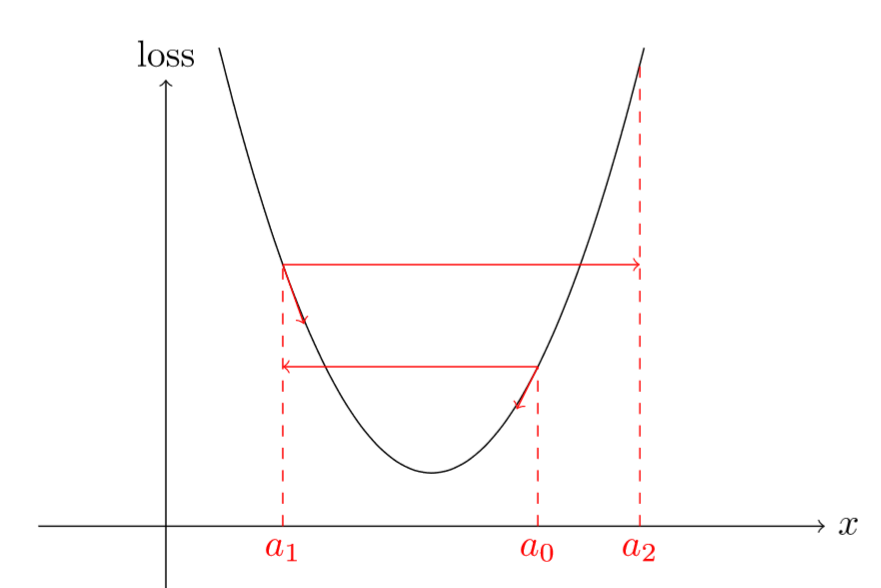
\includegraphics[width=8cm]{fig/f7.png}
    \caption{损失函数的梯度下降示意图}
    \label{f7}
\end{figure}

因此在表(\ref{learning_rate})中,当学习率过大时,会使损失函数不收敛,导致准确率断崖式下跌,使网络丧失识别功能。

学习率的选取在网络学习中是很重要的,直接关系到网络的性能,在此简单介绍一下学习率的的选取方法。
\begin{figure}[htbp]
    \centering
    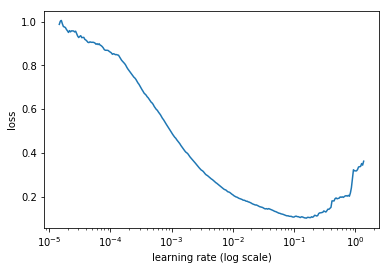
\includegraphics[width=8cm]{fig/f8.png}
    \caption{学习率和损失函数的函数关系}
    \label{f8}
\end{figure}
如图(\ref{f8})所示,可以尝试不同的初始学习率,然后可以以5至10轮的训练为标准,比较最终学习效果。一般学习率可以从$0.1\sim 10^{-8}$或者更大的范围去搜索,可以每次缩小10倍,这样做的好处是,可以快速的找到一个能够快速收敛的学习率。\newline

一些流行的学习率调整方法有:
\begin{itemize}
    \item 循环学习率:
    
    如图(\ref{f9})所示的三角学习率方法,蓝色线条代表学习率在上下限之间进行变化,输入参数\textit{stepsize} (步长) 是半个周期内的迭代次数。  
    \begin{figure}[htbp]
        \centering
        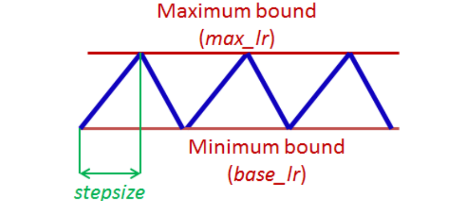
\includegraphics[width=10cm]{fig/f9.png}
        \caption{循环学习率示意图}
        \label{f9}
    \end{figure}

    \item 热启动的随机梯度下降(SGD):
    
    循环学习率是讲述的总体学习率调节技巧,然而如果我们不使用预训练的网络,我们应该如何开始我们的网络学习过程呢,就有学者提出热启动的概念。即在刚开始网络经过初始化之后,需要经过一定的调整之后才能达到一个快速学习的状态,需要经过一些柔性的学习率调节之后就能达到一个更加好的初始化状态,这可看作是对网络初始化的一个补充。
\end{itemize}

\subsubsection{改变卷积核步长(Stride)}
初始化程序\colorbox[gray]{0.9}{\texttt{Seq\_CNN\_course}}中卷积层的步长(Stride)为1,运行程序得到训练时间为27571.64ms,预测时间为1502.56ms,正确率为95.78\%。

改变程序\colorbox[gray]{0.9}{\texttt{Seq\_CNN\_course}}中卷积层的步长(Stride),将步长改为2,运行程序,得到训练时间为6657.11ms,预测时间为412.14ms,正确率为10.28\%。



可见,更改步长后训练时间从原来的27571.64ms变为6657.11ms,易知$27571/6657\approx 4$,这和步长变为原来的两倍是一致的。且更改步长后,网络丧失数字识别能力,可见选取合适的步长是非常重要的,否则会导致网络遗漏掉图片中的信息,不能学习到参数。

将步长改为3,则出现了错误:Segmentation fault (core dumped),将步长改为4,也出现了同样的错误。


\subsubsection{池化层调参}

改变池化层窗口大小,统计训练时间及准确率,见下表(\ref{pool})所示。

\begin{table}[htbp]
    \centering
    \caption{改变池化层窗口大小,训练时间及准确率的统计}
    \label{pool}
    \begin{tabular}{c|cccccc}
        \hline
        窗口大小&1&2&3&4&5&10\\
        \hline
        训练时间(ms)&26366.30&27739.95&28699.36&28904.23&30576.52&31098.66\\
        准确率(\%)&92.44&94.58&92.03&88.19&86.37&84.59\\
        \hline
    \end{tabular}
    
\end{table}

通过表(\ref{pool})可以看到,随着池化层窗口的增大导致训练时间边长,同时准确率也下降,从90\%以上下降至85\%以下,这是符合预期的。

首先解释时间增大的原因,此池化层是最大池化层,且在池化窗口中寻找最大值时采用双重for循环,因此随着池化窗口的增大,增大的最大值寻找的时间,导致最终训练时间增大;再解释准确率下降的原因,由于采用最大池化层,因此在增大池化层窗口的过程中,会丢失更多的信息,导致准确率下降,一般池化窗口采用$2\times 2$大小。

池化层的介绍见前文。

\subsection{运行速度的比较}

在本节,主要对训练的速度进行一个比较,比较GPU并行和一般程序的运行速度,并对CUDA编程进行介绍。


在程序\colorbox[gray]{0.9}{\texttt{Seq\_CNN\_course}}中,设置学习率为$0.01\sqrt{240}$,设置训练集共250个批次,每个批次的大小为240张图片,因此共$240\times 250=60000$个图片作为训练集,同时将10000张图片作为测试集,运行5次程序,记录每次的训练时间和测试时间。同时设置\colorbox[gray]{0.9}{\texttt{Cuda\_CNN\_ptr}}中的参数同上,并运行5次,记录每次的训练时间和测试时间,得到结果如下表(\ref{train_time})所示。


\begin{table}[htbp]
    \centering
    \caption{训练时间和测试时间比较}
    \label{train_time}
    \begin{tabular}{c|ccccc}
        \hline
        次数&1&2&3&4&5\\%&6&7&8&9&10\\
        \hline
        无GPU并行时训练时间(ms)&27571.64&27292.08&27287.97&27314.55&27315.76\\
        无GPU并行时测试时间(ms)&1502.59&1504.26&1506.38&1505.95&1505.32\\
        \hline
        有GPU并行时训练时间(ms)&267.58&267.69&267.08&267.79&267.28\\
        有GPU并行时测试时间(ms)&41.83&41.80&48.27&49.28&48.59\\
        \hline
    \end{tabular}
\end{table}



从表(\ref{train_time})可以看到,有GPU并行时的程序的运行效率大大提高,训练时间是无GPU并行的$1/100$,测试时间是无GPU并行的$1/33$。效率大大提高。



\section{实验感想}


在本次课程设计中,我学到了非常多的东西,主要有以下几点:
\begin{enumerate}
    \item 详细了解学习了卷积神经网络的相关知识。
    \item 学习到了卷积神经网络的组成,主要由卷积层、池化层,归一化层,全连接层组成。虽然在之前对此稍有了解,但本次的研究加深了对此的了解,为以后的工作打下了基础。
    \item 对网络的参数进行了调整并观察比较结果,学习到了网络超参数对网络的性能有至关重要的影响。
    \item 同时,学习到了一些调参的基本技巧。
    \item 了解并学习了CUDA编程。
    \item 体会到的CUDA编程在深度学习中的重要地位。
    \item 除了关于深度学习的知识外,本次课程设计,加深了我对C++语言的理解,并增强了我阅读代码和写代码的能力。
    

\end{enumerate}

本次课程设计中,我收获颇丰,在未来的学习工作生活中,我会加倍努力,增强自身素养,包括但不限于程序编写能力,论文撰写能力,发现问题的能力,提出问题的能力,解决问题的能力,英语能力等各方面能力。希望在未来的学习科研工作生活中,平衡好各方面关系,达到自己的目标。

\end{document}